\documentclass[a4paper]{article}

% Packages
\usepackage{listings}
\usepackage{color}
\usepackage[utf8]{inputenc}
\usepackage{listingsutf8}
\usepackage{graphicx}
\usepackage{epstopdf}
\usepackage{fancyhdr}
\usepackage[T1]{fontenc}
\usepackage{pmboxdraw}
\usepackage{parskip}
%\usepackage[top=2cm, bottom=2cm, left=3.5cm, right=2cm]{geometry} % Les marges.
\usepackage[top=2cm, bottom=2cm, left=2cm, right=2cm]{geometry} % Les marges.

\definecolor{mygreen}{rgb}{0,0.6,0}
\definecolor{mygray}{rgb}{0.5,0.5,0.5}
\definecolor{mymauve}{rgb}{0.58,0,0.82}
\definecolor{bggray}{rgb}{0.95, 0.95, 0.95}
\lstset{inputencoding=utf8/latin1}
\lstset{ %
    backgroundcolor=\color{bggray},   % choose the background color; you must add \usepackage{color} or \usepackage{xcolor}
    basicstyle=\footnotesize,        % the size of the fonts that are used for the code
    breakatwhitespace=false,         % sets if automatic breaks should only happen at whitespace
    breaklines=true,                 % sets automatic line breaking
    captionpos=b,                    % sets the caption-position to bottom
    commentstyle=\color{mygreen},    % comment style
    deletekeywords={...},            % if you want to delete keywords from the given language
    escapeinside={\%*}{*)},          % if you want to add LaTeX within your code
    extendedchars=true,              % lets you use non-ASCII characters; for 8-bits encodings only, does not work with UTF-8
    frame=single,                    % adds a frame around the code
    frameround=tttt                  % tttt for having the corner round.
    keepspaces=true,                 % keeps spaces in text, useful for keeping indentation of code (possibly needs columns=flexible)
    keywordstyle=\color{blue},       % keyword style
    language=Matlab,                 % the language of the code
    morekeywords={*,...},            % if you want to add more keywords to the set
    numbers=left,                    % where to put the line-numbers; possible values are (none, left, right)
    numbersep=5pt,                   % how far the line-numbers are from the code
    numberstyle=\tiny\color{mygray}, % the style that is used for the line-numbers
    rulecolor=\color{black},         % if not set, the frame-color may be changed on line-breaks within not-black text (e.g. comments (green here))
    showspaces=false,                % show spaces everywhere adding particular underscores; it overrides 'showstringspaces'
    showstringspaces=false,          % underline spaces within strings only
    showtabs=false,                  % show tabs within strings adding particular underscores
    stepnumber=1,                    % the step between two line-numbers. If it's 1, each line will be numbered
    stringstyle=\color{mymauve},     % string literal style
    tabsize=2,                       % sets default tabsize to 2 spaces
    title=\lstname                   % show the filename of files included with \lstinputlisting; also try caption instead of title
}

% Header
\pagestyle{fancy}
\fancyhead[L]{Axel Fahy \& Rudolf Höhn}
\fancyhead[R]{\today}


\title{Mini-projet - Snake multiplayer\\Réseaux I}
\author{Axel Fahy \& Rudolf Höhn}
\date{\today}


\begin{document}
\maketitle

\section{Introduction}
Ce projet consiste à implémenter 3 couches de protocoles de communication réseau imbriquées au-dessus d'UDP pour rendre multijoueur une version graphique (mise à disposition) du jeu Snake. Les 3 couches sont celles-ci :
\begin{itemize}
\item \textbf{SnakeChannel} : Cette couche s'occupe principalement de deux tâches. La première est la circulation de données, elle permet d'avoir l'assurance que le message reçu est plus récent que le dernier message traîté. La deuxième tâche est celle de la connexion, à travers une suite de messages hors-bande, elle atteste que la personne qui nous envoie des données est connue.
\item \textbf{SnakePost} : Cette couche nous permet d'envoyer des messages avec accusé de réception, dits fiables. Elle nous atteste que le destinataire a bien reçu notre message.
\item \textbf{SnakeGame} : La dernière couche est la couche de jeu, c'est elle qui s'occupe de toute la logique applicative. C'est le payload qui transite à travers SnakePost et SnakeChannel. Dans ce protocole, le serveur gère les collisions entre joueurs, la nourriture des serpents et les scores. C'est le maître du jeu.
\end{itemize}

\section{Architecture globale}
\begin{verbatim}
.
├── Client
│   ├── banner.py
│   ├── constants.py
│   ├── data/
│   ├── object_foods.py
│   ├── object_snake.py
│   ├── preferences.py
│   ├── scores.py
│   ├── snake_client.py
├── constants.py
├── doc/rapport/
├── Server
│   ├── constants.py
│   ├── player.py
│   ├── snake_server.py
├── snake_channel
│   ├── client_channel.py
│   ├── constants.py
│   ├── __init__.py
│   ├── server_channel.py
│   └── snake_channel.py
├── snake_post
│   ├── client_post.py
│   ├── client_post_udp.py
│   ├── constants.py
│   ├── __init__.py
│   ├── server_post.py
│   ├── server_post_udp.py
│   └── snake_post.py
└── timer
    ├── __init__.py
    └── timer.py
\end{verbatim}
\section{Fonctions, structures de données et objets/modules/classes}

\section{Fonctionnalités et bugs}



\section{Machines d'état}
\subsection{SnakeChannel émetteur}
\begin{center}
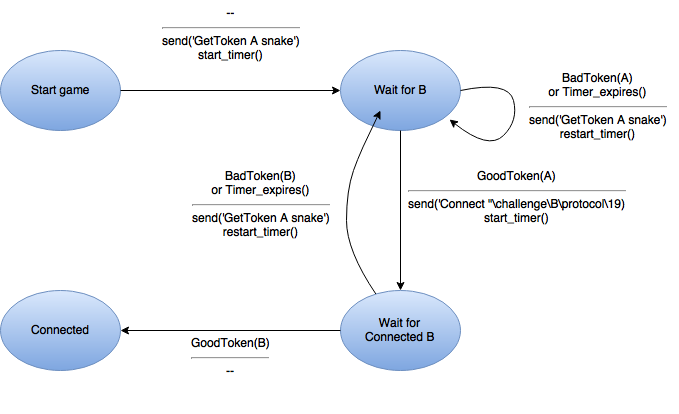
\includegraphics[scale=0.7]{sc_emetteur.png}
\end{center}
\subsection{SnakeChannel récepteur}
\begin{center}
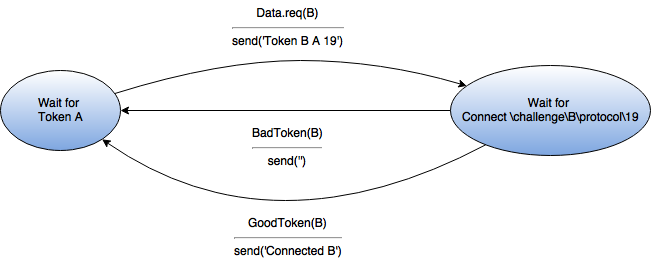
\includegraphics[scale=0.7]{sc_recepteur.png}
\end{center}
\subsection{SnakePost émetteur}
\begin{center}
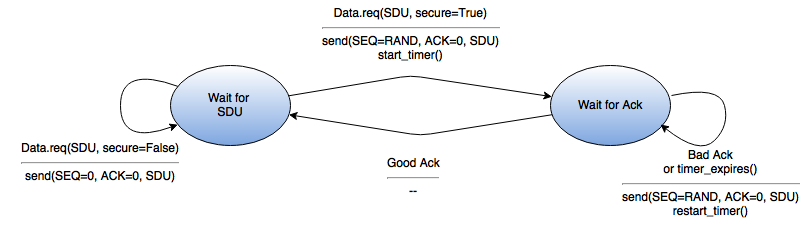
\includegraphics[scale=0.6]{sp_emetteur.png}
\end{center}
\subsection{SnakePost récepteur}
\begin{center}
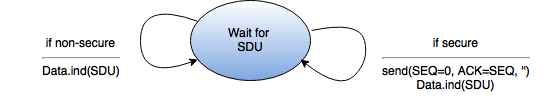
\includegraphics[scale=0.7]{sp_recepteur.png}
\end{center}

A rajouter dans le rapport :
- meme nom : deny connection
- probleme avec le serveur du prof, on recoit jamais rien
- snakeChannel : si le client est deja connecte, il va essayer de se connecter a l'infini
- on recommence tout a zero si jamais se pass mal a la connexion (SC)


\end{document}


